\documentclass[10pt]{article}
\usepackage[polish]{babel}
\usepackage[utf8]{inputenc}
\usepackage[T1]{fontenc}
\usepackage{amsmath}
\usepackage{amsfonts}
\usepackage{amssymb}
\usepackage[version=4]{mhchem}
\usepackage{stmaryrd}
\usepackage{graphicx}
\usepackage[export]{adjustbox}
\graphicspath{ {./images/} }

\title{LIGA MATEMATYCZNA \\
 im. Zdzisława Matuskiego \\
 LISTOPAD 2014 \\
 SZKOŁA PODSTAWOWA }

\author{}
\date{}


\begin{document}
\maketitle
\section*{ZADANIE 1.}
Oblicz sumé cyfr liczby \(10^{50}-2014\).

\section*{ZADANIE 2.}
Do trzech samochodów należy zapakować pięć pojemników wypełnionych do pełna farbą, pięć takich pojemników wypełnionych farbą do połowy i pięć pustych pojemników. Należy je zapakować tak, aby każdy samochód został jednakowo obciążony. Jak to zrobić?

\section*{ZADANIE 3.}
W pudełku są drewniane klocki w trzech różnych kolorach. Klocków niebieskich i zielonych razem jest 50, zielonych i czerwonych łacznie jest 40, niebieskich i czerwonych - 68. Oblicz ile jest klocków każdego koloru.

\section*{ZADANIE 4.}
Z 500 kwadratów o obwodzie 20 cm każdy, ułożono prostokąt, którego długość jest pięć razy większa od szerokości. Wyznacz pole i obwód otrzymanego prostokąta.

\section*{ZADANIE 5.}
Każdą z liczb 1, 2, 3, 4, 5 należy wpisać w wolne pola figury przedstawionej na rysunku tak, aby sumy liczb w wierszu i kolumnach były takie same. Na ile sposobów można to zrobić?\\
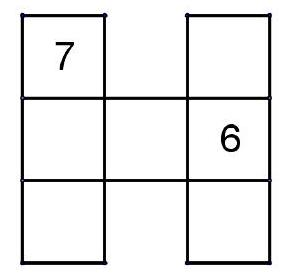
\includegraphics[max width=\textwidth, center]{2024_11_21_406b3b78e649b3e15709g-1}


\end{document}